% Pursuing Stacks (cotes 134-2 to 134-8): archive cote 134-4, site page 6 (PDF page 7), typescript page 94.
% typescript. Draft compared: ps3.tex:261-330.
% AI-transcribed by Claude Opus 5.5 (claude-opus-5-5, adaptive thinking, effort high), Message Batches API, batch ps1 (msgbatch_01Rv5hCaNTtUt4JHx1yqoHPL), 2026-11-12; image review recorded in records/CHECK_DECISIONS_134_3_4.tsv.
\scanpage{134-4/6}
\mspage{(94)}

I can now state the ``interesting extra feature'' \unsure{a}
\uline{Observation} For a functor $i: A\hand{\to} M$ of a weak test category A into the
modelizer M (with final object $e_M$ , giving rise to the final object in
$H_M = W_M^{-1}M$), and in the special case when M = (Cat), the following condi-%
tions are equivalent:
(i) $i^*$ transforms weak equivalences into weak equivalences , i.e.
induces a functor \deleted{\xout{$\unsure{H_A = W_A^{-1}A^{\hand{\wedge}}}$}} $H_M\hand{\to} H_{A^{\hand{\wedge}}}$\hand{\unsure{.}}
(ii) $i^*$ transforms aspheric objects into aspheric objects.
(iii) i is a weak test functor, namely $W_M = i^{*\,-1}(W_{A^{\hand{\wedge}}})$ (a stronger
version of (i)) \uline{and} the induced functor $H_M\hand{\to} H_{A^{\hand{\wedge}}}$ is an
\uline{equivalence}.

Here the obvious implications are of course
\[ \text{(iii)} \hand{\Longrightarrow} \text{(i)} \hand{\Longrightarrow} \text{(ii)} , \]
the second implic\hand{\ensuremath{\smile}}ation coming from the fact that $i^*$ is compatible with
final objects, and that $e_{A^{\hand{\wedge}}}$ is aspheric. Of course, (ii) means that
for any aspheric x in M , $A_{\hand{/}i^*(x)}$ is aspheric in (Cat). In case M =
(Cat), and when moreover the elements i(a) in (Cat) have final objects
(a condition I forgot to include in the statement of the observation
above, sorry), this condition was seen to imply (iii) (cf. ``key result''
on p.61 , \xout{condition a(iv)}\inserted[typed]{(a iv)\hand{$\Rightarrow$}(a ii)}) - indeed, it is even enough to check that
\deleted{Ax} for any C \uline{with final element} in \hand{(}Cat) , $i^*(C)$ is aspheric. T\over[typed]{H}{h}e proof
moreover turns out practically trivial, in terms of the usual asphericity
criterion for a functor between categories. So much so that the really
amazing strength of the statement, which appears clearly when looked at
in a more general setting\xout{\unsure{,}} as I just did, was kind of blurred by the
impression of \inserted{merely} fastiduously grinding through routine equivalences. We got
\margin{\diagram{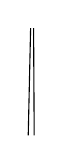
\begin{tikzpicture}[x=1ex,y=1ex]\draw (0,0)--(.2,9);\draw (.5,0)--(.45,9);\end{tikzpicture}}} there at any rate quite an interesting class of functors between modelizers
(an elementary and the basic one, for the time being\hand{)}, for which the
mere fact that the functor be compatible with weak equivalences, or only
even take aspheric objects into aspheric ones, implies that the functor
is modelizing, namely that the functor $H_M\hand{\to} H_{A^{\hand{\wedge}}}$ it induces (and the
very \uline{existen\over{c}{c}e} of this functor was all we demanded \inserted{beforehand!}) is actually an \uline{equi-}%
\uline{valence of categories}.

T\over{h}{h}e question that immediately \hand{\unsure{.}}comes to mind now, is if this ``extra
feature'' is indeed an extremely special one, strongly dependant on the
assumptions M = (Cat) and the categories i(a) having final objects -
or if it may not have a considerably wider significance. This suggests
the still more general questions, involving two modelizers M,M' , nei-%
ther of which needs be elementary \hand{or} \inserted{be}\hand{ (Cat) itself:}

\margin{6}
